BLEビーコンの基地局の位置情報を基に初期進行方向の補正を行ったが
常にそれが利用可能であるとは限らない.
電波を使った手法としてWi-Fiを使った手法もあるがこの場合も同様であり
基地局の位置情報の把握にはコストがかかる場合がある.
基地局の位置情報を用いない代替手法としてFPを用いた手法がある.
この手法は,事前に特定の場所で受信したBLEビーコンのIDと
電波強度のデータを蓄積しておく必要があり,そのデータを基に
受信したIDとRSSIの値から位置を推定する.
この手法を用いて初期進行方向を補正する関数を
Listing\ref{lst:rotate-trajectory-using-ble-fingerprint}に示す.
この関数は引数に加速度DF,角度データDF,BLEビーコンの受信電波DF,
BLEビーコンのFPDF,フロア名を受け取る.
戻り値は角度DFと座標DFを返す.
受信電波情報とFPを基に推定した座標を示したのが図\ref{fig:fingerprint-location}である.
図の青色の点が受信したBLEビーコンの基地局座標であり,
赤色の点がこの基地局から受信した電波とFPを基に位置を推定した座標である.
理解しやすいように図中では受信したIDが1つのみを表示しているが,
実際は複数の強い電波を受信した点が存在する.
また説明のために基地局情報を示しているが今回の使用ケースでは
この座標は判明していないのが前提である.
この関数の内部処理では上記で示した受信電波情報とFPを基に推定した座標と
推定軌跡の座標との距離の総和を用いて,
その和が最小となる角度を探す.
BLEビーコンの基地局情報を基に初期進行方向を回転させた際と,ほぼ同様の結果が得られた.


\begin{table}[ht]
	\centering
	\begin{tabular}{lll}
		\toprule
		カラム名        & 単位      & データ型  \\
		\midrule
		ts          & s (秒)   & float \\
		x           & m(メートル) & float \\
		y           & m(メートル) & float \\
		z           & m(メートル) & float \\
		bdaddress   & なし      & str   \\
		rssi        & dBm     & int   \\
		floor\_name & なし      & str   \\
		\bottomrule
	\end{tabular}
	\caption{BLEビーコンFPのDF}
	\label{table:ble-beacon-fingerprint-df}
\end{table}


\begin{figure}[ht]
	\centering
	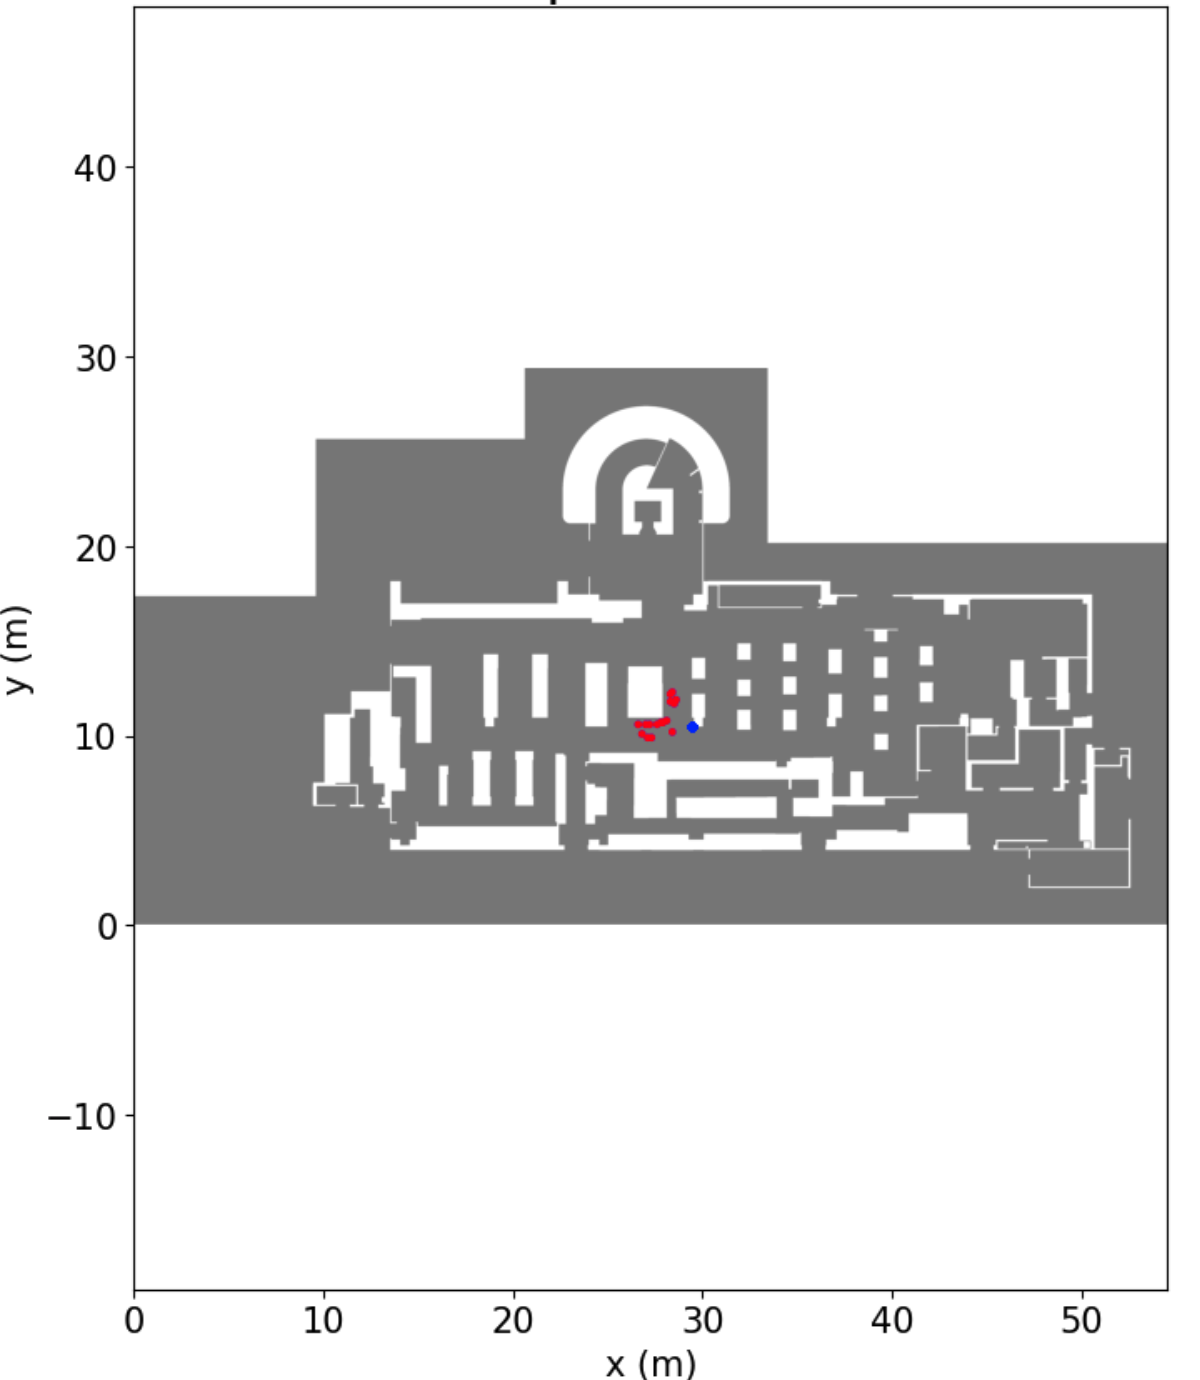
\includegraphics[width=80mm]{image/fingerprint-location.jpg}
	\caption{FPに基づく位置の推定}    \label{fig:fingerprint-location}
\end{figure}


\begin{figure}[ht]
	\centering
	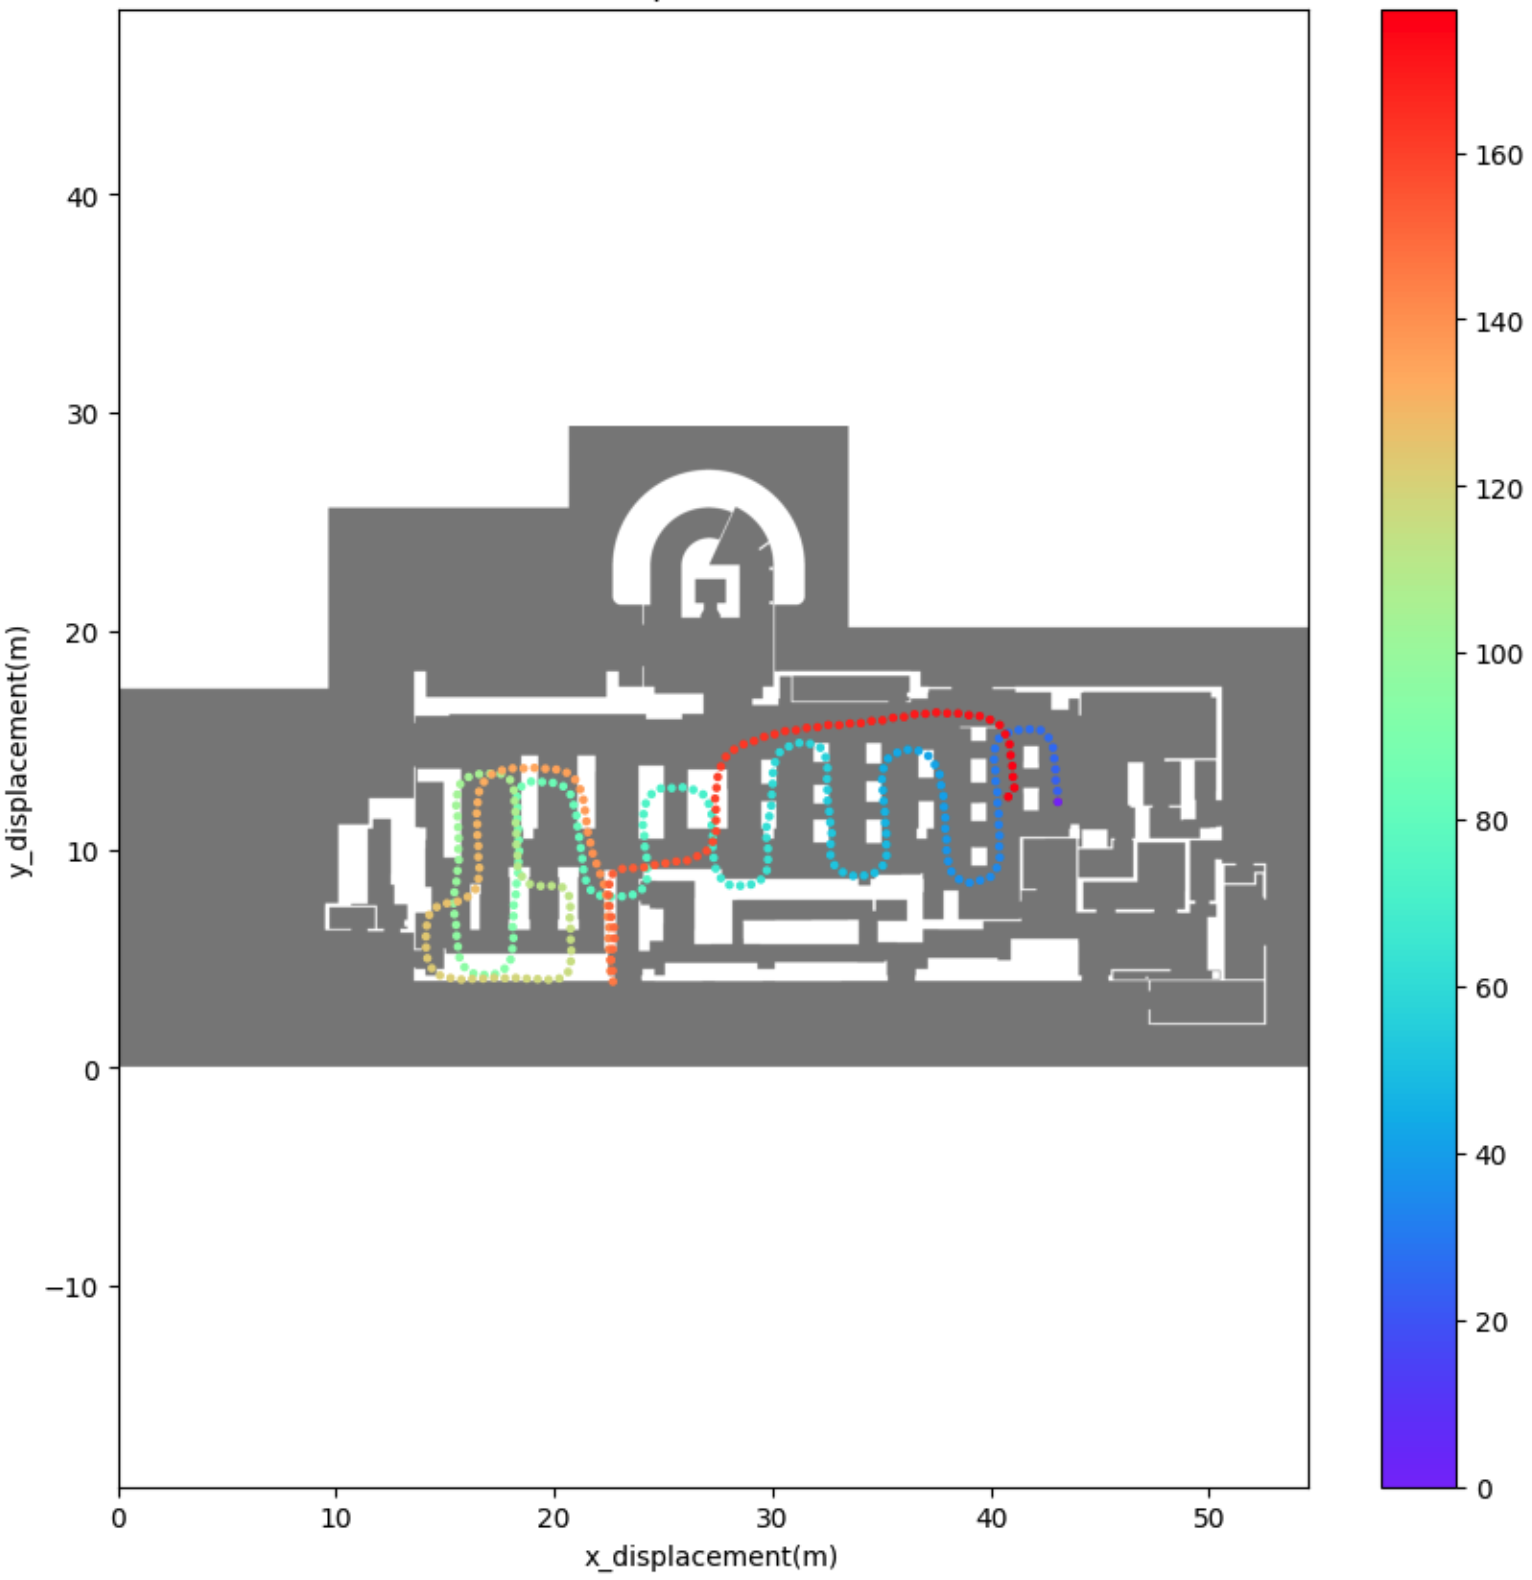
\includegraphics[width=80mm]{image/fingerprint-rotate.jpg}
	\caption{BLEのFPを補正後の軌跡}    \label{fig:fingerprint-rotate}
\end{figure}

\begin{lstlisting}[caption={BLEビーコンのFPを使用した\\初期進行方向補正}, label=lst:rotate-trajectory-using-ble-fingerprint]
def rotate_trajectory_to_optimal
          _alignment_using_ble_fingerprint(
    acc_df: pd.DataFrame,
    angle_df: pd.DataFrame,
    ble_scans_df: pd.DataFrame,
    ble_fingerprint_df: pd.DataFrame,
    floor_name: str,
    *,
    ground_truth_first_point: dict[Axis2D, float] | None = None,
) -> tuple[pd.DataFrame, pd.DataFrame]:                                        
\end{lstlisting}
